\section{Wstęp}

\begin{frame}
  $$ f(x) = \sum_{i=0}^m a_i \cdot x^i = 0; \qquad a_m \neq 0 $$

  \begin{itemize}
    \item Wielomian stopnia $m$, $m$ pierwiastków,
    \item $a_i$ rzeczywiste -- ewentualne pierwiastki zespolone są parami sprzężone:
    $$ \alpha + \textit{\textrm{i}} \cdot \beta, \quad \alpha - \textit{\textrm{i}} \cdot \beta $$
    \item $a_i$ zespolone -- brak związku między pierwiastkami.
  \end{itemize}
\end{frame}

\begin{frame}
  Szukanie zer:
  \begin{itemize}
    \item W zasadzie dowolną metodą,
    \item ze względu na postać $f(x)$ -- metody specjalne (zwłaszcza dla zespolonych)
  \end{itemize}

  Trudności:
  \begin{itemize}
    \item Krotne pierwiastki -- trudno ,,obramować'', łatwiej, gdy znana krotność,
    \item Blisko położone pierwiastki -- trudności jak wyżej.
  \end{itemize}

  \textit{Nie wiadomo z góry, jaki typ patologii wykazuje wielomian.}

  \vspace{5px}

  \textbf{Ważne:} \textit{Zadanie wyznaczania zer wielomianów może być źle uwarunkowane} (Wilkinson).
  % Czymkolwiek/kimkolwiek nie byłby Wilkinson
\end{frame}

\begin{frame}
  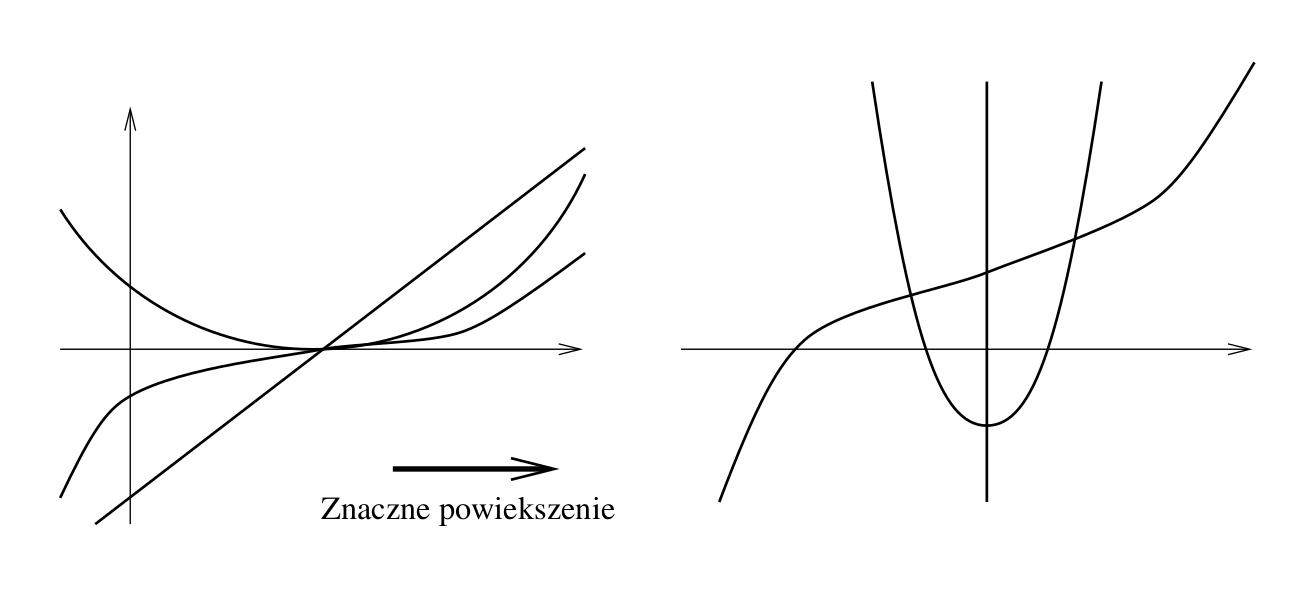
\includegraphics[width=\textwidth]{img/8/wielomian}
\end{frame}
